%%Énoncé
Énoncez précisément le problème résolu par l’algorithme de Knuth-Morris-Pratt
présenté dans le livre de référence. Quelle est la complexité temporelle de cet algorithme et grâce à quoi est-elle meilleure que celle de l’algorithme Brute Force ?
Justifiez vos réponses.
\\

%%Réponse
L'algorithme de Knuth-Morris-Pratt (KMP) résout le problème posé par l'implémentation de l'algorithme Brute Force: pour chaque index candidat de \textit{T} (la chaine de caractères de longueur \textit{n} dans laquelle on souhaite savoir si le pattern \textit{P}, de longueur \textit{m}, est présente), on parcours les \textit{m} caractères qui suivent pour vérifier si ils matchent \textit{P}. Si ce n'est pas le cas, on passe à l'index suivant de \textit{T} et on recommence à partir du début de \textit{P}.
La complexité temporelle de cet algorithme est en $O(n m)$.
Le problème est donc que l'on teste tous les caractères du pattern \textit{P} à chaque fois alors qu'il y a potentiellement des séquences de caractères identiques au sein même de \textit{P}.\\
\begin{figure}[h]
	\centering
	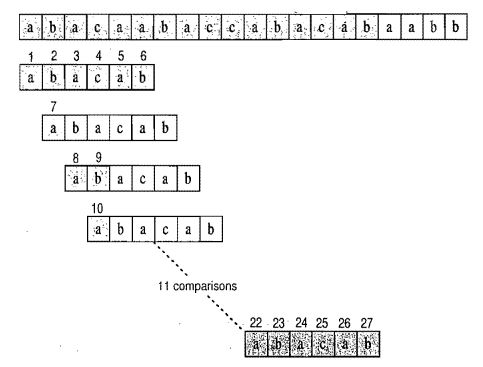
\includegraphics[scale=1]{q2-brute-force.jpg}
	\caption{Exemple de Brute Force pattern matching}
	\label{fig:bruteforce}
\end{figure}
La figure \ref{fig:bruteforce} \footnote{Issue du livre de référence DSAJ-5 page 565} est un exemple de l'algorithme de pattern matching de Brute Force. On peut voir qu'un total de 27 comparaisons est nécessaire pour trouver un résultat. On remarque bien que lorsqu'un caractère de \textit{P} ne correspond pas au caractère de \textit{T}, la comparaison reprend au premier caractère de \textit{P} et au caractère suivant de \textit{T}.
			 

L'algorithme KMP propose de pré-compiler le pattern \textit{P} en calculant une \textit{failure function} qui indiquera pour chaque caractère à quel endroit de \textit{P} recommencer la comparaison échoue.
\begin{figure}[h]
	\centering
	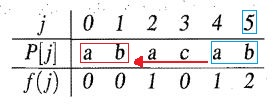
\includegraphics[scale=1]{q2-failure-function2.jpg}
	\caption{Exemple du résultat produit par \textit{failure function} pour le pattern \textit{a b a c a b}}
	\label{fig:failurefunction}
\end{figure}
La figure \ref{fig:failurefunction}\footnote{Issue du livre de référence DSAJ-5 page 570} nous montre que pour le pattern \textit{a b a c a b}, si la comparaison $T[i] == P[j]$ échoue, quand \textit{j} est égal à 5, il n'est pas nécessaire de recomparer les valeurs 0 et 1 pour \textit{j}.

\begin{figure}[h]
	\centering
	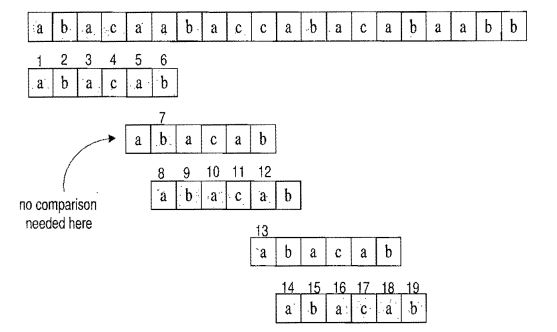
\includegraphics[scale=1]{q2-kmp.jpg}
	\caption{Exemple de l'algorithme de pattern matching Knuth-Morris-Pratt}
	\label{fig:kmp}
\end{figure}

La figure \ref{fig:kmp}  \footnote{Issue du livre de référence DSAJ-5 page 572} est un exemple d'exécution de l'algorithme de Knuth-Morris-Pratt avec les mêmes valeurs pour \textit{T} et \textit{P} que sur la figure \ref{fig:bruteforce}. On peut voir ici que 19 itérations sont nécessaires au lieu des 27 précédentes.

La complexité temporelle de cet algorithme est $O(n+m)$ avec \textit{n} égal à la longueur de la chaine \textit{T} et \textit{m} égal à la longueur du pattern \textit{P}.
Pourquoi cette complexité ? Parce que le calcul de la fonction d'erreur (\textit{failure function}) s'exécute en $O(m)$ et qu'ensuite le parcours de \textit{T} s'exécute en $O(n)$.

Cette complexité temporelle est meilleure que celle de l'algorithme de Brute Force car cette dernière valait potentiellement $O(n^2)$ si $m = n/2$. Alors que pour l'algorithme de KMP, elle vaut $O(n+m)$ dans le pire des cas.
